\documentclass[10pt,a4paper]{article}

\usepackage[margin=2.1cm]{geometry}
\usepackage[T1]{fontenc}
\usepackage{newtxtext,newtxmath}
\usepackage{booktabs}
\usepackage{graphicx}
\usepackage{subcaption}
\usepackage{array}
\usepackage{multirow}
\usepackage{amsmath}
\usepackage{xcolor}
\usepackage{tikz}
\usetikzlibrary{positioning,arrows.meta,fit,backgrounds,calc,shapes.geometric}
\usepackage[colorlinks=true,linkcolor=blue!55!black,citecolor=blue!55!black,
            urlcolor=blue!55!black]{hyperref}
\usepackage[numbers,sort&compress]{natbib}
\usepackage{caption}
\captionsetup{font=small,labelfont=bf,width=0.95\linewidth}
\usepackage{titlesec}
\titlespacing*{\section}{0pt}{1.1ex plus .3ex}{0.6ex}
\titlespacing*{\subsection}{0pt}{0.9ex plus .2ex}{0.4ex}

\definecolor{cData}{HTML}{56B4E9}
\definecolor{cGen}{HTML}{E69F00}
\definecolor{cModel}{HTML}{0072B2}
\definecolor{cStack}{HTML}{009E73}
\definecolor{cFail}{HTML}{B0B0B0}
\definecolor{cAccent}{HTML}{D55E00}

\newcommand{\auc}{ROC-AUC}
\newcommand{\dlt}[1]{$#1\times10^{-4}$}

\title{\vspace{-1.2cm}\bfseries How the Top Ten Solved Playground S6E10\\[2pt]
\large A Survey of Winning Pipelines: Generative Scorers, Public OOF Stacks,\\
and What the Final Leaderboard Actually Rewarded}
\author{The Time Forever \quad (Kaggle: \textsf{adamsmith1112})\\[2pt]
\small Companion to \emph{Where the Gains Come From}; Kaggle Playground S6E10}
\date{November 2026}

\begin{document}
\maketitle

\begin{abstract}
\noindent
We read every public write-up of the ten highest-placed teams in Kaggle Playground S6E10
(airline satisfaction, 699{,}635 training rows, \auc) and reconstruct what they built.
Five of the ten published solutions, one only in outline; the remaining five can be seen
only through their leaderboard footprint. Two grammars account for all of them. The first models the
joint distribution of a row and its label, classifies by Bayes' rule, and wins because the
competition data were themselves sampled from a language model fitted to the original
airline survey: a 124M-parameter GPT-2 that reads the label \emph{first} reaches 0.96242
out-of-fold on its own, more than any GBDT, tabular foundation model or 250-column stack.
The second grammar stacks a shared pool of public out-of-fold predictions with a strongly
regularised logistic regression; on its own it saturates at $0.9624$ --- exactly where 126
teams tie on the final private board. The winning margin came from adding a handful of
generative members to such a stack, not from more trees. We quantify this with the final
public and private leaderboards (four of the five best public entries collapsed), tabulate the
self-reported gains of each ingredient, and close with the validation discipline that the
top teams shared. Our companion study reported 0.96133 private from an eight-family blend;
this survey explains the remaining $1.2$--$1.9\times10^{-3}$.
\end{abstract}

\section{Scope, sources and what can be verified}
\label{sec:scope}

Playground competitions end with a leaderboard and, if the community is generous, with
write-ups. S6E10 ended on 31 October 2026 with 3{,}734 teams and an unusual amount of
shared material: several teams published not only their pipelines but also the
out-of-fold (OOF) predictions that other teams then stacked, and two of the strongest
solutions are written as tutorials~\citep{kaggle_first,kaggle_qft,kaggle_qft2}.

This document is a survey, not a reproduction. Its claims come from three sources, each
with a different strength of evidence:
\begin{enumerate}
  \item \textbf{The final leaderboards.} We downloaded the public board (all 3{,}735 rows)
        and the private top 200 with the Kaggle CLI; every number in
        Section~\ref{sec:board} is computed from those files.
  \item \textbf{The published solutions.} Discussions 754683 (1st), 754814 (4th),
        754643 (5th), 754646 (7th), 754641 (9th), 754666 (11th), 754658 (16th),
        754782 (25th), 755475 (28th) and 754691 (29th) are the primary sources for the
        methods; all are cited as blog-style references, because that is what they are.
  \item \textbf{The shared code.} Two of the tutorials include runnable notebooks and
        prediction datasets, and the 7th-place team documents its file contract.
\end{enumerate}
Teams 2, 3, 6, 8 and 10 published nothing, so their rows in Table~\ref{tab:board} are
markers only; we do not guess at their pipelines.

\paragraph{Relation to our own run.}
The companion paper~\citep{kaggle_s6e10} (this repository) documents a controlled ladder of
feature, family and ensemble interventions on the same folds, ending at 0.960901
cross-validated and 0.96133 private (rank 1{,}536). That study deliberately avoided the
public-prediction ecosystem and the generator. This survey covers exactly the two things it
left out, which is why it can name the mechanism behind the remaining gap.

\section{The board the winners were playing}
\label{sec:board}

Table~\ref{tab:board} lists the final top ten together with their public standing.
The private board reordered almost everything: the winner was seventh on public, the
third-place team eleventh, the fourth fourteenth, while the public leader was not in the
private top 200 at all.

\begin{table}[t]
\centering
\small
\caption{Final private leaderboard (top ten) with the same teams' public standing.
``Public'' is the best public submission each team recorded, so a team can appear higher
there than the file that produced its private score. Team 10 and 11 tie at five decimals.}
\label{tab:board}
\begin{tabular}{rlrrrl}
\toprule
\# & Team & public rank & public \auc{} & private \auc{} & public write-up\\
\midrule
1  & Chris Deotte              & 7   & 0.96261 & 0.96318 & yes \citep{kaggle_first}\\
2  & Prior (3 members)         & 9   & 0.96252 & 0.96308 & no\\
3  & Christoffer Thimsen       & 11  & 0.96241 & 0.96306 & no\\
4  & Ole-Jakob                 & 14  & 0.96236 & 0.96304 & yes \citep{kaggle_fourth}\\
5  & Abdelrahman mohsen        & 10  & 0.96242 & 0.96292 & yes (short) \citep{kaggle_fifth}\\
6  & srikalyan                 & 12  & 0.96238 & 0.96280 & no\\
7  & UIT --- Loc \& An         & 403 & 0.96213 & 0.96263 & yes \citep{kaggle_seventh}\\
8  & Maher el Ouahabi          & 541 & 0.96199 & 0.96262 & no\\
9  & Fritz Cremer              & 8   & 0.96260 & 0.96259 & yes \citep{kaggle_ninth}\\
10 & Vivillon                  & 37  & 0.96226 & 0.96254 & no\\
\midrule
--- & this repository (8-family blend) & 1{,}204 & 0.96062 & 0.96133 & ---\\
\bottomrule
\end{tabular}
\end{table}

\subsection{The public board was a different game}

Figure~\ref{fig:lb} (left) plots public against private score for the 200 teams whose
private score we can see. Three facts stand out.

\emph{The public top five mostly vanished.} Public scores above 0.963 were achieved by five
teams; four of them (0.96473, 0.96451, 0.96375, 0.96319) do not appear in the private top
200, and the fifth fell to 58th (0.96239). The public board is 30\% of the test set, so it
is noisier than the private one --- but only by about $\sqrt{70/30}\approx1.5$ in standard
error. That cannot explain a $10^{-3}$ gap; fitting the 30\% can.

\emph{Everyone else moved up, by the same amount.} 99\% of the private top 200 scored
higher on private than on public, with a mean shift of \dlt{4.2}
(Figure~\ref{fig:lb}, right). Our submission shows the same constant offset
(0.96062 $\to$ 0.96133, \dlt{7.1}). The offset is a property of the split, not of a team.

\emph{Above 0.9623 the board is a tie.} The private scores from rank 75 onward are all
0.96238: 126 of the first 200 rows share that value. That is not 126 independent
discoveries; it is the same column of public OOF predictions stacked with slightly
different code and submitted at the same granularity. The cheap part of this competition
was over long before the deadline.

The consequence for reading the rest of this document: differences of \dlt{1} among the
top teams are mostly selection noise, while differences of \dlt{5} and more are structural.
The two grammars below differ by more than that.

\begin{figure}[t]
\centering
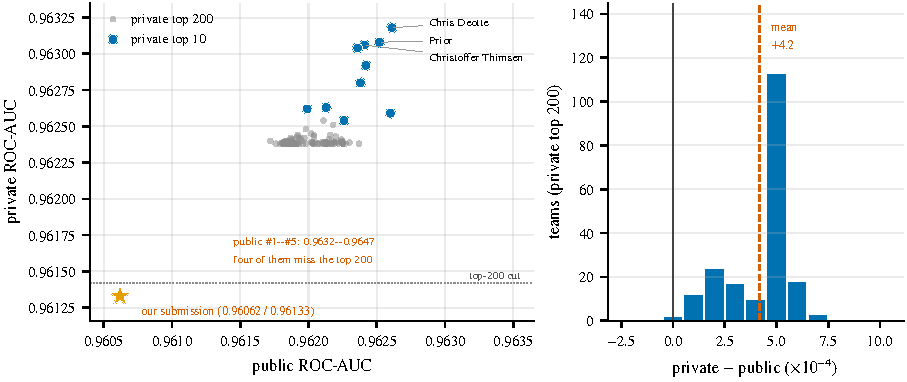
\includegraphics[width=\linewidth]{figures/fig_lb.pdf}
\caption{Left: public versus private score for the 200 teams whose private score is
visible. The top four public entries are off this axis to the right; four of the public
top five are absent from the private top 200. Right: distribution of the private$-$public
difference for the same teams (mean \dlt{+4.2}). The horizontal band of grey points on the
left is the 0.96238 tie. Our submission is marked for scale.}
\label{fig:lb}
\end{figure}

\section{The decisive fact: the rows were written by a language model}
\label{sec:generator}

The 1st-place write-up opens with a claim that reorganises the whole competition: the
training rows were sampled from GReaT~\citep{borisov2023greaT}, a GPT-2 fine-tuned on the
original 129{,}880-row airline survey, and the target is written \emph{before} the
features. Three independent checks support it.

\emph{Tokenizer fingerprints.} In the generated columns, a three-digit flight distance is a
single GPT-2 token while a four-digit distance is two tokens sharing a prefix --- exactly
what byte-level BPE does to numbers, and not what a tabular generator would do.

\emph{Sampling parameters.} A temperature of 0.7 with top-$k=50$ reproduces the distortions
the data show: departure delays collapse onto zero (mean 1.18 minutes against 14.71 in the
original survey) while the tail is truncated. The 29th-place team fitted a temperature per
column and recovered $T\approx0.7$ on both high-cardinality columns, with the
Kullback--Leibler divergence to the synthetic marginal falling from 0.308 to 0.004 for the
delay column~\citep{kaggle_twentyninth}. Our own audit reached the same delay collapse from
the other direction, without knowing its cause.

\emph{The prior is reproduced exactly.} Conditioning on \texttt{satisfaction is True}
first and sampling forward reproduces the 44.36\% positive rate of the training set. A
generator that writes the label last cannot do that.

\subsection{Two ways to read a row}

If the data are $p(y)\,p(x\mid y)$, the Bayes-optimal classifier is not the discriminative
$p(y\mid x)$ that everyone trains; it is the likelihood ratio
\begin{equation}
\log\frac{p(y{=}1\mid x)}{p(y{=}0\mid x)}
= \log\frac{\pi}{1-\pi}
+ \sum_{j=1}^{21}\Big[\log p(x_j\mid x_{<j},y{=}1)-\log p(x_j\mid x_{<j},y{=}0)\Big],
\label{eq:bayes}
\end{equation}
with $\pi=0.4436$ estimated on the training rows. Figure~\ref{fig:directions} contrasts the
two readings. The \emph{detective} appends the target and reads it from the last position:
one forward pass per row, but it is a classifier trained on 700k rows, and it reaches only
$\approx0.961$. The \emph{storyteller} runs the same model twice, once per label, and adds
the log-probabilities of the observed features: the label is never predicted, only scored.
No feature tokenizer, no architecture change, no extra data --- a stock GPT-2 with the
right prompt direction.

\begin{figure*}[t]
\centering
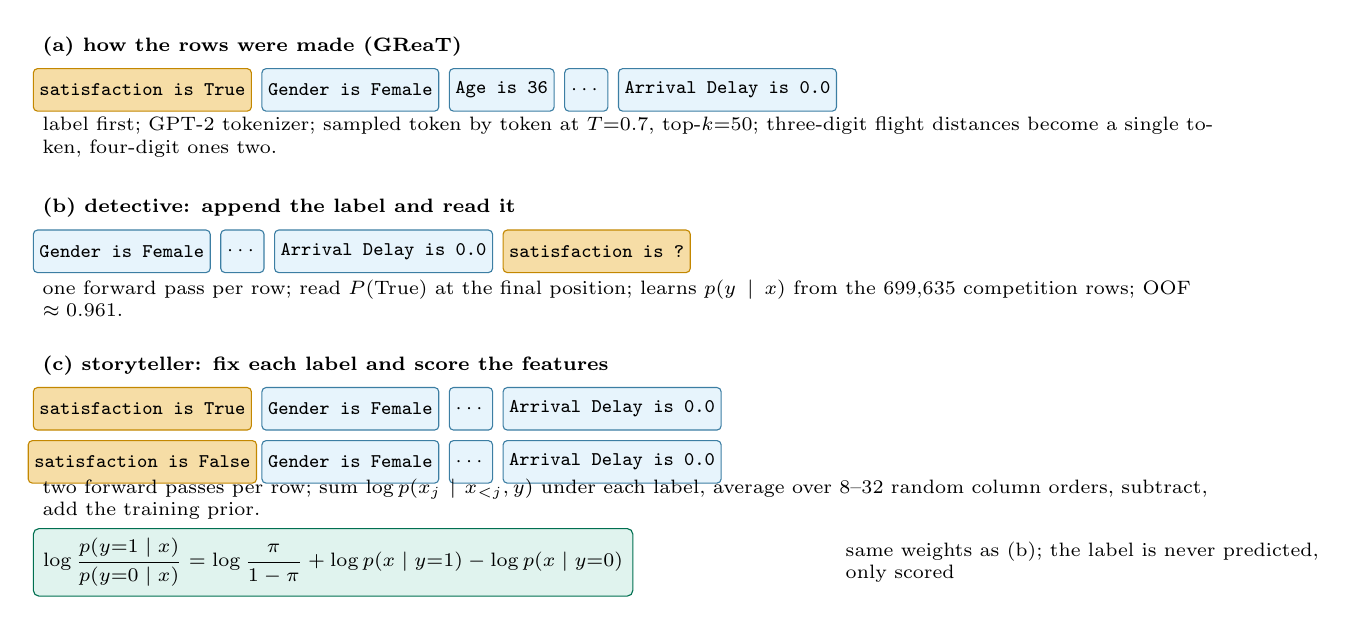
\begin{tikzpicture}[
  font=\scriptsize,
  cell/.style={draw, rounded corners=1.5pt, inner sep=2.2pt, minimum height=5.4mm,
               line width=0.4pt, fill=white, anchor=west},
  lab/.style={cell, fill=cGen!35, draw=cGen!85!black},
  feat/.style={cell, fill=cData!14, draw=cData!70!black},
  note/.style={anchor=west, align=left, font=\scriptsize, text width=150mm},
  head/.style={anchor=west, font=\scriptsize\bfseries},
]
% ---- (a) generation -------------------------------------------------------
\node[head] at (0,0) {(a) how the rows were made (GReaT)};
\node[lab]  (g1) at (0,-0.55) {\texttt{satisfaction is True}};
\node[feat, right=1.2mm of g1] (g2) {\texttt{Gender is Female}};
\node[feat, right=1.2mm of g2] (g3) {\texttt{Age is 36}};
\node[feat, right=1.2mm of g3] (g4) {$\cdots$};
\node[feat, right=1.2mm of g4] (g5) {\texttt{Arrival Delay is 0.0}};
\node[note] at (0,-1.15)
  {label first; GPT-2 tokenizer; sampled token by token at $T{=}0.7$, top-$k{=}50$;
   three-digit flight distances become a single token, four-digit ones two.};

% ---- (b) detective --------------------------------------------------------
\node[head] at (0,-2.05) {(b) detective: append the label and read it};
\node[feat] (d1) at (0,-2.6) {\texttt{Gender is Female}};
\node[feat, right=1.2mm of d1] (d2) {$\cdots$};
\node[feat, right=1.2mm of d2] (d3) {\texttt{Arrival Delay is 0.0}};
\node[lab, right=1.2mm of d3] (d4) {\texttt{satisfaction is ?}};
\node[note] at (0,-3.2)
  {one forward pass per row; read $P(\text{True})$ at the final position; learns
   $p(y\mid x)$ from the 699{,}635 competition rows; OOF $\approx0.961$.};

% ---- (c) storyteller ------------------------------------------------------
\node[head] at (0,-4.05) {(c) storyteller: fix each label and score the features};
\node[lab]  (s1) at (0,-4.6) {\texttt{satisfaction is True}};
\node[feat, right=1.2mm of s1] (s2) {\texttt{Gender is Female}};
\node[feat, right=1.2mm of s2] (s3) {$\cdots$};
\node[feat, right=1.2mm of s3] (s4) {\texttt{Arrival Delay is 0.0}};
\node[lab,  below=1.2mm of s1] (s5) {\texttt{satisfaction is False}};
\node[feat, below=1.2mm of s2] (s6) {\texttt{Gender is Female}};
\node[feat, below=1.2mm of s3] (s7) {$\cdots$};
\node[feat, below=1.2mm of s4] (s8) {\texttt{Arrival Delay is 0.0}};
\node[note] at (0,-5.75)
  {two forward passes per row; sum $\log p(x_j\mid x_{<j},y)$ under each label, average
   over 8--32 random column orders, subtract, add the training prior.};

\node[draw, rounded corners=2pt, fill=cStack!12, draw=cStack!70!black, inner sep=3.5pt,
      font=\scriptsize, anchor=west] (eq) at (0,-6.55)
  {$\displaystyle
   \log\frac{p(y{=}1\mid x)}{p(y{=}0\mid x)}
   =\log\frac{\pi}{1-\pi}+\log p(x\mid y{=}1)-\log p(x\mid y{=}0)$};
\node[anchor=west, font=\scriptsize, text width=62mm] (eqnote) at (10.2,-6.55)
  {same weights as (b); the label is never predicted, only scored};
\end{tikzpicture}
\caption{The generator and the two ways to interrogate it. (a) Rows were sampled from a
GPT-2 fine-tuned on the original survey, with the label written first. (b) The obvious
classifier appends the label and reads it; it learns $p(y\mid x)$ from 700k rows.
(c) The winning direction writes each label first, scores the features under both labels,
and combines them with the training prior; the label is never predicted. Both (b) and (c)
use the same network.}
\label{fig:directions}
\end{figure*}


\subsection{How much the direction is worth}

Table~\ref{tab:generative} collects the numbers published by the teams. The ordering is
consistent across three independent implementations: discriminative reading $\approx0.961$;
generative scoring $0.9620$--$0.9625$; and the difference survives when the generative model
is a from-scratch transformer rather than GPT-2, which rules out ``GPT-2 memorised the
original survey'' as the whole explanation.

\begin{table}[t]
\centering
\small
\caption{Single-model \auc{} for the generative family, as reported by the teams.
``OOF'' is out-of-fold on the shared five-fold split.}
\label{tab:generative}
\begin{tabular}{lll}
\toprule
Model & OOF \auc{} & Source\\
\midrule
GPT-2 small, target last (discriminative)      & 0.9610            & \citet{kaggle_first}\\
Q-FT v2 (ModernBERT encoder, set reading)      & 0.96080           & \citet{kaggle_qft2}\\
AO-ARM, best single recipe                     & 0.96201           & \citet{kaggle_fourth}\\
GenPure, one seed (6 layers, width 256)        & 0.96119           & \citet{kaggle_seventh}\\
GPT-2 medium / large, target first             & 0.96237 / 0.96236 & \citet{kaggle_first}\\
GPT-2 small, target first                      & 0.96242           & \citet{kaggle_first}\\
GPT-2 small, target anywhere                   & 0.96245           & \citet{kaggle_first}\\
\bottomrule
\end{tabular}
\end{table}


\section{Two grammars for the top of the board}
\label{sec:systems}

Every published solution is a combination of two components: \emph{generative members},
which supply the structural signal of Section~\ref{sec:generator}, and a \emph{stack}, which
supplies variance reduction. The mixture explains the shape of Table~\ref{tab:board}: the
winner used both; the 4th place used only generative members and no public predictions; the
7th, 11th and 16th put a generative family on top of a large public stack; and the 25th,
28th and 29th ran stacks of discriminative members alone, landing at 0.9624.

\begin{figure}[t]
\centering
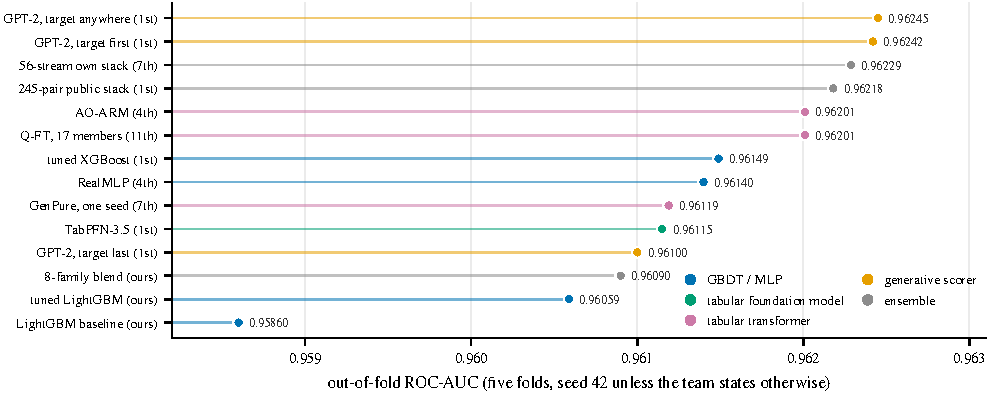
\includegraphics[width=\linewidth]{figures/fig_ladder.pdf}
\caption{Single-model \auc{} on the shared folds, as reported by the teams. Bars are drawn
from 0.9582 to the value; colour marks the model family. The row marked ``ours'' is this
repository's eight-family blend, i.e.\ what a conventional pipeline reaches. Every
generative scorer except the discriminative reading sits above it, and the best one is a
124M GPT-2.}
\label{fig:ladder}
\end{figure}

\subsection{Generative members: four implementations of one idea}

\paragraph{GPT-2 with the target first (1st).}
A stock GPT-2 small is fine-tuned for 60 epochs on the original survey and 8 epochs on the
competition rows, with the columns in random order; at prediction time 30 random orders are
combined with a log-sum-exp. Formatting follows the original file exactly (integer age,
one-decimal delays, \texttt{None} for missing), the GPT-2 tokenizer is used rather than a
digit-wise one, and cases are left as in the source. Ten such members (small, medium and
large backbones, target first/anywhere, plus a GPT-Neo variant) carry about 80\% of the
final stack's output~\citep{kaggle_first}.

\paragraph{AO-ARM (4th).}
A from-scratch encoder replaces GPT-2: every column value becomes a learned embedding
(column embedding plus value embedding, with a separate vocabulary per column), the model
is an any-order autoregressive transformer, and classification is the averaged
log-likelihood difference over 32 random column orders, one model per fold. Twenty-one
AO-ARM streams carry about 70\% of the net standardised coefficients of a 189-stream
logistic stack, and one recipe alone scores 0.96258 on private~\citep{kaggle_fourth}.

\paragraph{GenPure (7th).}
Twenty-one tokens per row from a vocabulary built on train and test features only; numeric
values seen fewer than three times are merged into coarse bins. A 6-layer, 256-wide,
8-head causal transformer models $P(x,y)$ with a new random column order per batch; the
score is the log-mean-exp of the Bayes log-odds over eight fixed orders. Unlabelled rows
(train-test and held-out folds) contribute a feature-likelihood term with weight 0.5, and
each fold gets Platt scaling on a 10\% inner holdout, which also picks the epoch. Two
choices mattered: pure generative training (adding a BCE term on the log-odds lowered OOF
from 0.95960 to 0.95907) and training longer (12 $\to$ 36 epochs, +0.0016 per seed,
early stopping off)~\citep{kaggle_seventh}.

\paragraph{Q-FT and Q-FT v2 (shared by 1st, 9th, 11th).}
Q-FT feeds 22 learned vectors per row (21 features plus a CLS) into a frozen Qwen3-0.6B
decoder through LoRA, with column embeddings initialised from the word vectors of the column
names, per-value lookup tables that include one entry per flight-distance ``route'', and
periodic numeric embeddings~\citep{kaggle_qft}. Version~2 replaces the decoder with a
bidirectional ModernBERT encoder, sets every \texttt{position\_ids} to zero so the row is
read as a set, adds side features and two summary tokens, and pretrains on replaced-token
detection: 149M parameters, $6.5$ minutes per fold on one A100, OOF 0.960798 against Q-FT's
0.959795~\citep{kaggle_qft2,warner2024modernbert}. The 11th-place team's 17 Q-FT members
moved their stack from 0.96213 to 0.96241~\citep{kaggle_eleventh}.

\subsection{The stack: a shared pool and a regularised linear head}

The second component is boring on purpose. Every team converted probabilities to logits,
standardised them with statistics from the training part of the meta-fold, and fitted an
$L_2$ logistic regression; the differences are the pool and the shrinkage.

\begin{itemize}
  \item \textbf{Pool.} Public OOF/test pairs on the same five folds accumulated from 119
        columns on 6 October to 245 by 20 October and 284--531 by the deadline; teams
        deduplicated at a logit correlation of 0.999 and verified each file's row order and
        fold assignment. Figure~\ref{fig:pools} shows who used how much.
  \item \textbf{Shrinkage.} $C=0.3$ for a 56-column own-only stack, $C=0.003$ for 299--312
        columns, $C=0.01$ for 364. The 29th-place team reports that re-tuning $C$ from 0.1
        to 0.01 when their pool grew from 199 to 364 members was worth \dlt{0.3} --- more
        than any single new member they added later~\citep{kaggle_twentyninth}.
  \item \textbf{Non-linear heads are optional.} The 25th-place team averaged
        $0.8\,z(\text{LR})+0.2\,z(\text{LightGBM})$ over 299 columns; the 28th-place team
        tried an $L_1$ logistic (470 inputs, 173--192 non-zero coefficients per fold) and a
        CatBoost on logits initialised from a logistic margin. Both landed within
        \dlt{0.2} of plain $L_2$ logistic~\citep{kaggle_twentyfifth,kaggle_twentyeighth}.
\end{itemize}

\begin{figure}[t]
\centering
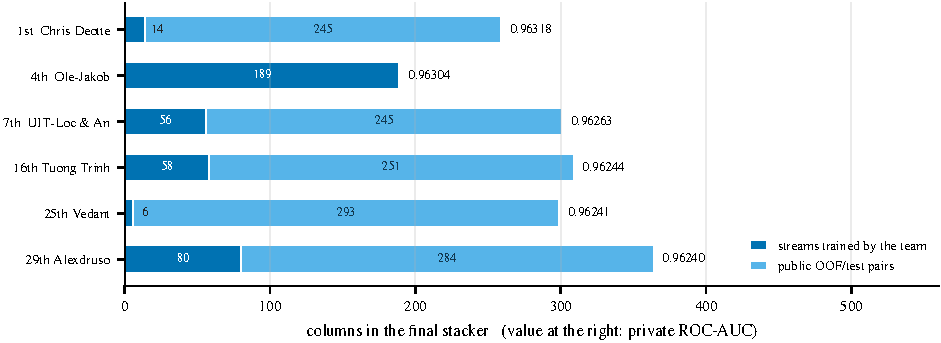
\includegraphics[width=\linewidth]{figures/fig_pools.pdf}
\caption{Composition of the final stacker for the six teams that state exact counts.
Blue: streams the team trained; light blue: public OOF/test pairs. Two routes reach the
top: 189 own streams and no public predictions (4th), or a handful of own generative
members plus the shared pool (1st). The number at the right of each bar is the private
\auc.}
\label{fig:pools}
\end{figure}

Table~\ref{tab:systems} summarises the published pipelines. The rightmost column is the
honest one: how much of each team's final score is attributable to a component that other
teams could not have copied from the public pool.

\begin{table}[t]
\centering
\small
\caption{Published solutions at a glance. ``Own'' and ``public'' count streams entering the
final stacker; ``CV'' and ``private'' are the team's own reported numbers.}
\label{tab:systems}
\begin{tabular}{p{2.05cm}p{1.8cm}p{7.95cm}rr}
\toprule
Team & own / public & ingredients, and what was new & CV & private\\
\midrule
1st Deotte & 14 / 245
  & GPT-2 $\times$10, nine TFMs, GBDTs. Target-first scoring on a GPT-2 fine-tuned on the
    original survey; ten such members carry most of the output
  & 0.96290 & 0.96318\\
4th Ole-Jakob & 189 / 0
  & AO-ARM $\times$21 plus XGBoost, RealMLP, CatBoost, TabPFN. Any-order transformer scored
    by likelihood; no public predictions used
  & 0.96279 & 0.96304\\
5th Mohsen & many / many
  & Not disclosed. Stack of own and shared OOF; CV-only selection in the final week
  & 0.96270 & 0.96292\\
7th UIT & 56 / 245
  & GenPure $\times$16 plus RealMLP, TabPFN, CatBoost, set transformers. Bagged generative
    transformer with Bayes scoring; two submission slots
  & 0.96247 & 0.96263\\
9th Cremer & $\approx$20 / 4
  & A pretrained transformer plus LightGBM, kNN and MLP. Masked-token and replaced-token
    pretraining on train$+$test
  & 0.96213 & 0.96259\\
11th Feng & 300+ / 3
  & XGBoost, LightGBM, CatBoost, RealMLP and 17 Q-FT members; 300-column $L_2$ logistic
  & 0.96241 & 0.96254\\
16th Trinh & 58 / 251
  & 42 feature-view GBDTs, TabPFN, a GPT-2 row classifier. GReaT surrogate likelihood ratios
    and a residual LightGBM on the offsets
  & --- & 0.96244\\
25th Singhal & 6 / 293
  & Six own members plus 293 community columns; 0.999 deduplication, LR/LightGBM 80/20
  & 0.96222 & 0.96241\\
29th Alexdruso & 80 / 284
  & LightGBM, RealMLP, kNN, EBM on feature views. Route-id target encoding; $C=0.01$ on 364
    columns
  & 0.96227 & 0.96240\\
\bottomrule
\end{tabular}
\end{table}


\section{What moved the needle, and what did not}
\label{sec:evidence}

The write-ups contain enough ablations to separate ingredients, although each was measured
against a different baseline. Table~\ref{tab:deltas} collects them in units of $10^{-4}$
\auc; the right-hand column names the measurement, because these are not interchangeable.

\begin{table}[t]
\centering
\small
\caption{Reported effects of individual ingredients, in \dlt{} of \auc. Numbers come from
different baselines and fold protocols, so compare magnitudes, not sums.}
\label{tab:deltas}
\begin{tabular}{p{5.6cm}p{2.2cm}p{5.2cm}}
\toprule
Ingredient & effect & measured as\\
\midrule
Route id (flight distance) with fold-safe target encoding, crosses and original-data
  per-route rates & $+15$ & single LightGBM, 5-fold \citep{kaggle_twentyninth}\\
First generative member added to a 245-column public stack & $+48$ & stack CV
  0.96218 $\to$ 0.96266 \citep{kaggle_first}\\
GReaT surrogate log-likelihood ratios from a distilgpt2 fitted on the original survey
  & $+28$ & standalone member \citep{kaggle_sixteenth}\\
Appending the original 129{,}880 rows (after route features) & $+2$ to $+3$
  & LightGBM / RealMLP \citep{kaggle_twentyninth}\\
Teacher logit trained on the original survey & $+2$ & LightGBM feature\\
Label-free auxiliary targets (predict each column from the other 20) & $+1$ & LightGBM feature\\
TabPFN-3.5 or TabICL members in a public-only stack & $+1$ & nested CV \citep{kaggle_publicstack}\\
Ten-fold instead of five-fold members & $+1$ & nested CV \citep{kaggle_publicstack}\\
Another GBDT or RealMLP member of the same kind & $+0.1$ to $+0.3$ & nested CV\\
Extra seeds of a generative transformer & $+0.7$, then $+0.8$, then $+0.1$
  & 3, 7 and 4 additional seeds \citep{kaggle_seventh}\\
SFS / hill-climbing instead of plain $L_2$ logistic & $-5$ to $-10$ on public, $+3$ on CV
  & 189-stream stack \citep{kaggle_fourth}\\
Blending 50/50 with the best public submission & $+190$ public, $-50$ private
  & 312-column stack \citep{kaggle_sixteenth}\\
Distilling from OOF predictions & $+50$ (leak) & matched leaky-vs-honest run
  \citep{kaggle_twentyninth}\\
Selecting the neural-network epoch on the scored fold & $+2$ (inflation) & RealMLP OOF
  \citep{kaggle_twentyninth}\\
\bottomrule
\end{tabular}
\end{table}

Three lessons follow from the table.

\emph{The generator is not another member.} Adding a good GBDT to a 250-column stack is
worth a third of a $10^{-4}$; adding one generative scorer is worth fifty. The reason is
visible in Figure~\ref{fig:ladder}: the members of the pool are all approximations of the
same conditional $p(y\mid x)$, so their errors are correlated, and a linear head can only
average them. A scorer of $p(x\mid y)$ makes mistakes on different rows --- which is also
why the 4th-place team could reach 0.96304 with no public predictions at all.

\emph{Feature work still matters, but only of one kind.} The largest single feature gain in
the whole competition is not a new model: it is treating \texttt{flight\_distance} as a
route identifier. It has 3{,}521 distinct values, all of which occur in the original survey;
per-route satisfaction rates correlate 0.87 with the original data, and a fold-safe target
encoding of that key (alone, then crossed with class, travel type and customer type) plus
the original per-route rate and route counts is worth \dlt{15} on a single LightGBM. The
original rows only help \emph{after} this feature exists, because each route then gains
about 37 labelled rows.

\emph{Everything else is inside the noise.} Seed averaging, extra folds, meta-learner
choice, calibration and most feature transforms stay below \dlt{2}. The 29th-place team ran
about twenty pre-registered experiments in the last two weeks --- new families (TabR,
ModernNCA, FT-Transformer, random-feature kernels), TFMs on their own features,
pseudo-labelling, six stacker variants --- and every honest result landed within
\dlt{1} of the stack. A large logistic stack absorbs ``another good model''.

\section{The part that is cheap to copy: validation discipline}
\label{sec:discipline}

Every top write-up spends more words on selection than on models, and the protocols are
nearly identical. Figure~\ref{fig:protocol} renders the consensus.

\begin{figure*}[t]
\centering
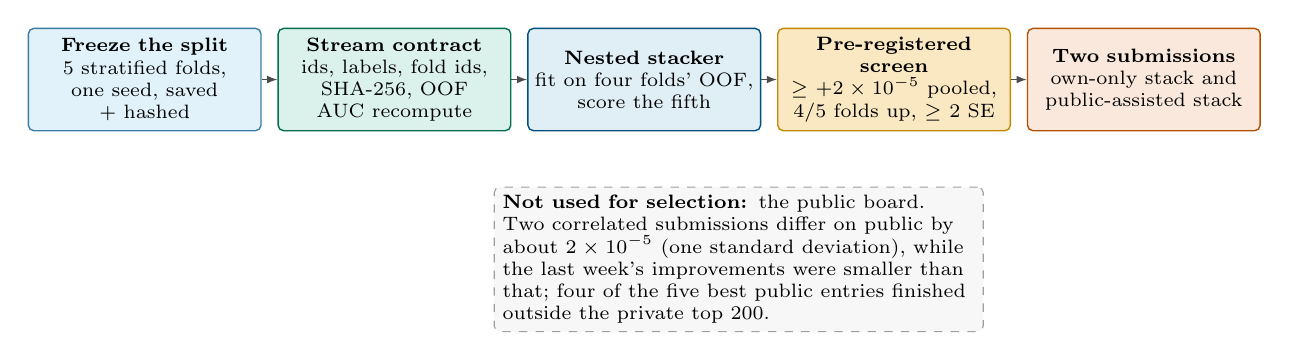
\begin{tikzpicture}[
  font=\scriptsize,
  stage/.style={draw, rounded corners=2pt, align=center, inner sep=2.2pt,
                minimum height=13mm, text width=28mm, line width=0.5pt},
  fold/.style={stage, fill=cData!18, draw=cData!70!black},
  check/.style={stage, fill=cStack!14, draw=cStack!70!black},
  meta/.style={stage, fill=cModel!12, draw=cModel!70!black},
  gate/.style={stage, fill=cGen!24, draw=cGen!85!black},
  sub/.style={stage, fill=cAccent!14, draw=cAccent!85!black},
  note/.style={draw=cFail!90!black, dashed, rounded corners=2pt, align=left,
               inner sep=3pt, text width=60mm, fill=cFail!10, font=\scriptsize},
  arr/.style={-{Latex[length=1.3mm]}, line width=0.5pt, draw=black!70},
  dasharr/.style={-{Latex[length=1.3mm]}, line width=0.5pt, draw=cFail!85!black, dashed},
]
\node[fold] (f) {\textbf{Freeze the split}\\5 stratified folds,\\one seed, saved + hashed};
\node[check, right=2mm of f] (c) {\textbf{Stream contract}\\ids, labels, fold ids,\\SHA-256, OOF AUC recompute};
\node[meta, right=2mm of c] (m) {\textbf{Nested stacker}\\fit on four folds' OOF,\\score the fifth};
\node[gate, right=2mm of m] (g) {\textbf{Pre-registered screen}\\$\ge +2\times10^{-5}$ pooled,\\4/5 folds up, $\ge 2$ SE};
\node[sub, right=2mm of g] (s) {\textbf{Two submissions}\\own-only stack and\\public-assisted stack};
\draw[arr] (f) -- (c);
\draw[arr] (c) -- (m);
\draw[arr] (m) -- (g);
\draw[arr] (g) -- (s);
\node[note, below=7mm of m, xshift=12mm] (n)
  {\textbf{Not used for selection:} the public board. Two correlated submissions differ on
   public by about $2\times10^{-5}$ (one standard deviation), while the last week's
   improvements were smaller than that; four of the five best public entries finished
   outside the private top 200.};
\end{tikzpicture}
\caption{The selection protocol shared by the top teams. The first three boxes make a
number honest; the fourth stops the team from chasing it; the fifth acknowledges that the
two candidate answers are different questions.}
\label{fig:protocol}
\end{figure*}

Four details are worth naming, because they are where most pipelines lose their CV:

\begin{enumerate}
  \item \textbf{A frozen split with a file contract.} The 7th-place team wrote every stream
        to the same layout (id, label, fold, OOF probability, test probability), then
        verified row order, label equality, fold equality, a producer-recorded SHA-256, and
        that the OOF \auc{} recomputes to $10^{-9}$. With 56--300 streams, one misaligned
        column is invisible in the total score but fatal to the stack.
  \item \textbf{Nested stacking.} The stacker is fitted on four folds' OOF and scored on
        the fifth, so the reported stack score is not the score of a model that saw its own
        validation rows. Teams that skipped this reported CV figures that did not transfer.
  \item \textbf{A screen fixed before the result.} The 7th-place threshold --- pooled gain
        $\ge 2\times10^{-5}$, at least four of five folds up, worst fold no worse than
        $-2\times10^{-5}$, mean gain at least two standard errors --- was written down
        before candidates were run. The 29th-place team pre-registered every experiment and
        reported the nulls.
  \item \textbf{A sealed holdout for the final claim.} The 16th-place team kept fold 0
        untouched (139{,}927 rows) and used paired DeLong standard errors
        \citep{deLong1988} on it for the last decisions, then submitted two files: an
        own-only stack and a public-assisted one.
\end{enumerate}

The counter-example is instructive. The 4th-place team's hill-climbing variant improved
cross-validated \auc{} by \dlt{3} over plain logistic regression but lost \dlt{5}--\dlt{10}
on public; the 16th-place team's 50/50 blend with the public leader gained \dlt{190} on
public and lost \dlt{50} on private. Both are the same phenomenon seen from two sides: with
300 correlated columns, a selection procedure with many degrees of freedom will fit the
30\% split, and the private board will charge for it.

\section{Discussion}
\label{sec:discussion}

\paragraph{Why a language model beats the models we usually tune.}
A GBDT on 21 columns learns a function of the marginals and a handful of interactions it
happens to split on. The data, however, were drawn from a joint distribution over 21
columns with strong dependence: delays, distance and cabin co-vary, and the generator
reproduces that joint at a temperature low enough to sharpen it. Scoring $p(x\mid y)$ uses
all of it, including the parts that do not predict the label but do constrain which rows
are plausible. The gap between 0.961 (discriminative GPT-2) and 0.9624 (same network, other
direction) is the value of that joint structure, not of scale: GPT-2 medium and large are
no better than small, while the direction is worth more than twenty times a new GBDT.

\paragraph{Is it a leak?}
No, and the write-ups are careful about it. The original survey is a public dataset that
the competition rules allow; fitting a density to it and applying Bayes' rule is a modelling
choice. The 4th-place result --- 0.96201 from a transformer trained from scratch on the
competition rows, with learned embeddings and no GPT-2 weights --- shows that the direction
matters even without the original corpus, and the 1st-place team re-ran the target-last
recipe on non-synthetic data and still beat XGBoost. What the generator gives is a prior
over rows; the competition still decides who estimates it best.

\paragraph{Why the stacks converge to 0.9624.}
Public OOF predictions are not independent evidence: they are many estimators of the same
conditional, trained on the same 700k rows, with the same features. A logistic head over
250 of them behaves like a very well-regularised average, and its ceiling is the ceiling of
that conditional. This is also why the private board ties at five decimals for 126 teams:
the differences that remain are the arbitrary ones.

\paragraph{Limitations of this survey.}
(i) We did not rerun any winning pipeline; every number in Sections~\ref{sec:generator}
and~\ref{sec:evidence} is self-reported, and the baselines differ (5 folds with different
seeds, different target encodings). (ii) Five of the top ten published nothing; we name
their reported backbones only where other write-ups credit them. (iii) Stack scores on
pooled public OOF are mildly optimistic, as the 25th-place team states explicitly: the
members were fitted on the same labels the stacker is scored against. (iv) The private
scores we use come from the leaderboard, whose ties at five decimals hide differences below
$10^{-5}$.

\paragraph{What generalises beyond this competition.}
Two practices transfer to any tabular problem. First, \emph{identify the data-generating
process before tuning}: here a tokenizer fingerprint and a temperature sweep cost an
afternoon and were worth \dlt{140} over the best conventional pipeline. Second, \emph{make
the validation honest enough to prefer a null result}: a frozen split, a file contract,
nested stacking and a pre-registered screen are cheap, and they are what separated the
teams that climbed from the teams that fell.

For our own repository, the actionable list is short: treat \texttt{flight\_distance} as a
route key with fold-safe target statistics (worth \dlt{15} on a single LightGBM in the
29th-place measurement), add a generative scorer as a member rather than as a replacement,
and re-tune the stacker's shrinkage whenever the pool grows.

\section{Reproducing this survey}
\label{sec:repro}

\begin{sloppypar}
Everything used here is public and was collected with the Kaggle CLI into
\texttt{artifacts/solutions/}: \texttt{leaderboard\_full.csv} (public board, 3{,}735 rows),
\texttt{leaderboard\_top200.csv} (private top 200), the ten write-ups as plain text under
\texttt{discussions/}, and one public stacking notebook. The two plotted figures are
produced by \texttt{paper/solutions/figures.py}; the two diagrams are TikZ in this
document.
\end{sloppypar}

\begin{verbatim}
kaggle competitions leaderboard playground-series-s6e10 -d
kaggle competitions leaderboard playground-series-s6e10 --show -v --page-size 200
kaggle competitions topics list playground-series-s6e10 --sort-by top
kaggle competitions topics show playground-series-s6e10 754683
python paper/solutions/figures.py
\end{verbatim}

Two practical notes for Windows users: the leaderboard archive contains a colon in its
entry name, so \texttt{Expand-Archive} refuses it and the CSV has to be extracted with
Python's \texttt{zipfile}; and the CLI prints Unicode minus signs, which requires
\texttt{PYTHONIOENCODING=utf-8} in a GBK console.

\appendix
\setlength{\emergencystretch}{2em}
\section{Recipe card for a generative scorer}
\label{app:recipe}

The following is the minimal version of the winning recipe, assembled from the four
published implementations. It assumes only a causal language model, no feature tokenizer
and no GPU cluster: GPT-2 small fits in 8\,GB and the five folds take a few hours on a
single mid-range GPU.

\begin{verbatim}
# 1. serialise a row exactly like the original file
text(row, y) = "satisfaction is {y}, " + ", ".join(f"{c} is {v}" for c, v in row)
               # integer age, one-decimal delays, "None" for missing

# 2. fit the generator on the original survey (129,880 rows)
model = GPT2small()
train_lm(model, [text(row, y) for row, y in original], epochs=60)

# 3. per fold: fine-tune, then score every validation and test row twice
for k in range(5):
    fold_model = train_lm(clone(model),
                          [text(row, y) for row, y in train if fold_id[row] != k],
                          epochs=8)
    for row in valid[k] + test:
        for y in (True, False):
            L[y] = mean_over_orders(sum_j log p_fold_model(x_j | x_<j, y))
        z[row] = log(pi / (1 - pi)) + L[True] - L[False]
\end{verbatim}

Four details decide whether this reproduces 0.9624 or 0.9610: (i) the label must come
\emph{first}; (ii) the serialisation must match the file the generator was trained on
(integer vs.\ float formatting, \texttt{None} for missing values); (iii) use a tokenizer
that keeps numbers compact --- GPT-2's, not a digit-wise one; and (iv) average the
log-likelihood difference over several column orders (8--32), which removes the arbitrary
order the model would otherwise memorise. The 7th-place team's variant replaces steps 2--3
with a from-scratch 6-layer transformer over per-column token vocabularies and keeps the
same scoring rule; the 4th-place variant does the same with 32 orders and a learned column
embedding. Both reach the same region, which is the strongest evidence that the direction,
not the backbone, is doing the work.

\sloppy
\bibliographystyle{plainnat}
\bibliography{references}


\end{document}

